\documentclass{../cshonours}
\usepackage{subfiles}
\usepackage{url}
\usepackage{graphics}
\usepackage{etoolbox}
\usepackage{bibunits}
\usepackage{amsfonts}
\usepackage{fixltx2e}
\usepackage{tabularx}
\usepackage{accsupp}
\usepackage{pifont}
\usepackage{abbrevs}
\usepackage{acronym}
\usepackage[vario]{fancyref}
\usepackage{threeparttable}
\usepackage{tikz}
\usepackage{hyperref}
\usepackage{xspace}
\usepackage{ccicons}
\usepackage{textcomp}
\usepackage{multicol}
\usepackage{enumerate}
\usepackage{rotating}
\usepackage{tabularx}
\usepackage{calc}
\usepackage{color}
\usepackage[chapter]{minted}
\usepackage{pdflscape}
\usepackage{upquote}
\usepackage{afterpage}
\usepackage{verbatim}
\usepackage{float}
\usepackage{rotfloat}
\usepackage{gensymb}
\usepackage{gnuplot-lua-tikz}
\usepackage{subcaption}
\usepackage{afterpage}

% Blank page command
\newcommand\blankpage{%
    \null
    \thispagestyle{empty}%
    \addtocounter{page}{-1}%
    \newpage}

% TODO: Change title
\newcommand{\thetitle}{Developing a robust system for occupancy detection in the household}
\newcommand{\theauthor}{Ash Tyndall}

\newcommand{\thekeywords}{keyword, keyword}
\newcommand{\thecategories}{category, category}

%%% BEGIN LATEX TWEAKS

% Tikz initialize
\usetikzlibrary{shapes, arrows, positioning, fit}
\tikzstyle{dashbox} = [rectangle, dashed, draw=black]
\tikzstyle{box} = [rectangle, draw=black, minimum width=3cm, minimum height=1cm, text centered, text width=3cm]
\tikzstyle{cbox} = [cloud, cloud puffs=15.7, minimum height=1cm, draw]
\tikzstyle{line} = [thin,-,>=stealth]
\tikzstyle{fbox} = [box, dotted, rounded corners=1mm]
\tikzstyle{fcont} = [rectangle, draw=black, minimum width=6cm, minimum height=2.5cm, text centered, text width=6cm]

% Check marks and cross marks
\newcommand{\cmark}{\hspace{7mm}\BeginAccSupp{ActualText=Y}\checkmark\EndAccSupp{}}
\newcommand{\xmark}{\hspace{7mm}\BeginAccSupp{ActualText=N}\ding{55}\EndAccSupp{}}
\newcommand{\ssup}{\textsuperscript{1}}
\newcommand{\tsup}{\textsuperscript{2}}

% Configure bibliography
\bibliographystyle{acm}
\defaultbibliography{../references/primary}
\defaultbibliographystyle{acm}

% Namelist stuff for proposal
\newcommand{\namelistlabel}[1]{\mbox{#1}\hfil}
\newenvironment{namelist}[1]{%1
\begin{list}{}
    {
        \let\makelabel\namelistlabel
        \settowidth{\labelwidth}{#1}
        \setlength{\leftmargin}{1.1\labelwidth}
    }
  }{%1
\end{list}}

% Additional table options
\newcommand*{\csbox}[1]{\parbox[c]{1.7cm}{\centering #1}}
\newcolumntype{"}{@{\hskip\tabcolsep\vrule width 1pt\hskip\tabcolsep}}

% Acronyms for common stuff
\newcommand{\acrodefn}[3]{%
	\acrodef{#1}[#2]{#3}%
	\expandafter\newcommand\csname#1\endcsname{\ac{#1}\xspace}%
}

\acrodefn{pir}{PIR}{Passive Infrared Sensor}
\acrodefn{iar}{IAR}{Infrared Array Sensor}
\acrodefn{mlx}{\textit{Melexis}}{Melexis MLX90620}
\acrodefn{emwa}{EMWA}{Exponential Weighted Moving Average}
\acrodefn{lowpan}{6LoWPAN}{IPv6 over Low power Wireless Personal Area Networks}
\acrodefn{coap}{CoAP}{Constrained Application Protocol}
\acrodefn{iot}{IoT}{Internet of Things}
\acrodefn{rest}{REST}{Representational state transfer}
\acrodefn{roll}{RPL}{IPv6 Routing Protocol for Low-Power and Lossy Networks}
\acrodefn{ws}{WS-*}{Web Services Descriptive Language / Simple Object Access Protocol}

% Abbreviation commands for common stuff
\newabbrev\cdi{CO\textsubscript{2}}
\newabbrev\lwifi{802.15.4}
\newabbrev\lmed{802.15.4e}
\newabbrev\lphy{802.15.4-2006}
\newabbrev\etal{et al.}
\newabbrev\iic{$\textrm{I}^2\textrm{C}$}
\newabbrev\ard{Arduino}
\newabbrev\geye{Grid-EYE}

% Misc commands
\newcommand{\dc}{\degree\textrm{C}}

% Fancyref support for subsections, source; https://github.com/openlilylib/tutorials/blob/master/aGervasoni/orchestralScores/example-materials/OLLbase.sty
\newcommand*{\fancyrefsubseclabelprefix}{subsec}

\fancyrefaddcaptions{english}{%
  \providecommand*{\frefsubsecname}{subsection}%
  \providecommand*{\Frefsubsecname}{Subsection}%
}

\frefformat{plain}{\fancyrefsubseclabelprefix}{\frefsubsecname\fancyrefdefaultspacing#1}
\Frefformat{plain}{\fancyrefsubseclabelprefix}{\Frefsubsecname\fancyrefdefaultspacing#1}

\frefformat{vario}{\fancyrefsubseclabelprefix}{%
  \frefsubsecname\fancyrefdefaultspacing#1#3%
}
\Frefformat{vario}{\fancyrefsubseclabelprefix}{%
  \Frefsubsecname\fancyrefdefaultspacing#1#3%
}

% Fancyref support for subsubsections, source; https://github.com/openlilylib/tutorials/blob/master/aGervasoni/orchestralScores/example-materials/OLLbase.sty
\newcommand*{\fancyrefsubsubseclabelprefix}{subsubsec}

\fancyrefaddcaptions{english}{%
  \providecommand*{\frefsubsubsecname}{subsection}% the same as for subsection
  \providecommand*{\Frefsubsubsecname}{Subsection}%
}

\frefformat{plain}{\fancyrefsubsubseclabelprefix}{\frefsubsubsecname\fancyrefdefaultspacing#1}
\Frefformat{plain}{\fancyrefsubsubseclabelprefix}{\Frefsubsubsecname\fancyrefdefaultspacing#1}

\frefformat{vario}{\fancyrefsubsubseclabelprefix}{%
  \frefsubsubsecname\fancyrefdefaultspacing#1#3%
}
\Frefformat{vario}{\fancyrefsubsubseclabelprefix}{%
  \Frefsubsubsecname\fancyrefdefaultspacing#1#3%
}

% Fancyref support for listings, source; http://tex.stackexchange.com/questions/70835/how-to-extend-fancyref-for-listings
\newcommand*{\fancyreflstlabelprefix}{lst}

\fancyrefaddcaptions{english}{%
  \providecommand*{\freflstname}{listing}%
  \providecommand*{\Freflstname}{Listing}%
}

\frefformat{plain}{\fancyreflstlabelprefix}{\freflstname\fancyrefdefaultspacing#1}
\Frefformat{plain}{\fancyreflstlabelprefix}{\Freflstname\fancyrefdefaultspacing#1}

\frefformat{vario}{\fancyreflstlabelprefix}{%
  \freflstname\fancyrefdefaultspacing#1#3%
}
\Frefformat{vario}{\fancyreflstlabelprefix}{%
  \Freflstname\fancyrefdefaultspacing#1#3%
}

% Enable subsubsections
\setcounter{secnumdepth}{3} % Enable level 4-5
\setcounter{tocdepth}{3}    % Include level 4-5 in TOC

% Reset acronym definitions in each section and chapter
\preto\section\acresetall
\preto\chapter\acresetall

% Hyperref setup
\hypersetup{pdftitle=\thetitle,pdfauthor=\theauthor,pdfsubject=\thecategories,pdfkeywords=\thekeywords,hidelinks}

% Square table config
\newcolumntype{z}[1] {
  @{{\centering \parbox[c]{\tabcolsep}{\rule{0pt}{#1 + 2\tabcolsep}}}}
  >{\centering\arraybackslash}
  m{#1} }
% 
\renewcommand{\tabularxcolumn}[1]{z{#1}}

% TOC in PDF bookmarks
\makeatletter
\usepackage{etoolbox}
\pretocmd{\tableofcontents}{%
  \if@openright\cleardoublepage\else\clearpage\fi
  \pdfbookmark[0]{\contentsname}{toc}%
}{}{}%
\makeatother

\makeatletter
\usepackage{etoolbox}
\pretocmd{\listoffigures}{%
  \if@openright\cleardoublepage\else\clearpage\fi
  \pdfbookmark[0]{\listfigurename}{lof}%
}{}{}%
\makeatother

\makeatletter
\usepackage{etoolbox}
\pretocmd{\listoftables}{%
  \if@openright\cleardoublepage\else\clearpage\fi
  \pdfbookmark[0]{\listtablename}{lot}%
}{}{}%
\makeatother

% Fix list of listings with minted
\renewcommand{\listoflistings}{%
  \cleardoublepage
  \addcontentsline{toc}{chapter}{\listoflistingscaption}%
  \listof{listing}{\listoflistingscaption}%
}

% Configure titles
\title{\thetitle}
\author{\theauthor}
\keywords{\thekeywords}
\categories{\thecategories}
%%% END LATEX TWEAKS

\begin{document}
\newcommand{\mainfile}{} % we use the existance of this command to see if we're compiling the whole thesis or just a chapter

\maketitle

\begin{abstract}
This is the abstract.
\end{abstract}

\newpage
\null
\vfill 
\noindent{\fontsize{40pt}{1em}\selectfont \ccbysa}

\null

\noindent\textcopyright\xspace 2014--15 Ashley Ben Tyndall

\noindent This document is released under a Creative Commons Attribution-ShareAlike 4.0 International License. A copy of this license can be found at \\ \url{http://creativecommons.org/licenses/by-sa/4.0/}.

\noindent A digital copy of this document and supporting files can be found at \\ \url{http://github.com/atyndall/honours}. % TODO: Change URLS to ash.id.au redirs

\noindent The following text can be used to satisfy attribution requirements:

\noindent ``This work is based on the honours research project of Ash Tyndall,  developed with the help of the School of Computer Science and Software Engineering at The University of Western Australia. A copy of this project can be found at \\ \url{http://github.com/atyndall/honours}.''
	
\noindent Code and code excerpts included in this document are instead released under the GNU General Public License v3, and can be found in their entirety at \\ \url{https://github.com/atyndall/thing}.

\newpage

\begin{acknowledgements}
These are the acknowledgements.

% TODO: Any thesis, dissertation or other publication resulting from research undertaken by the recipient while in receipt of the Hackett Foundation Alumni Honours Scholarship must acknowledge the support of the scholarship and carry the University by-line.
\end{acknowledgements}

\tableofcontents
\listoftables
\listoffigures
\listoflistings


\subfile{../introduction/introduction}
\subfile{../litreview/litreview}
\subfile{../design/design}
\subfile{../evaluation/evaluation}
\subfile{../conclusion/conclusion}

\addcontentsline{toc}{chapter}{Bibliography}
\bibliography{../references/primary}

\afterpage{\blankpage}

\appendix
\chapter{Physical Form}
% TODO: Add scale to photos
To enable the prototype to be easily mounted on the ceiling, the prototype was placed on a flat board with feet that would enable it to be screwed into a pole, and the pole extended to jam the sensor against the ceiling and the floor using the pole (\Fref{fig:pictures:protob1}, \Fref{fig:pictures:protoact}). Due to a wireless module and battery pack being added to the Raspberry Pi, it was feasible for the sensor to operate entirely wirelessly for several hours. However, in most cases it was more convenient to operate using wired power and Ethernet.

\begin{figure}[H]
\centering
\includegraphics[height=0.5\textheight]{../diagrams/prototype-mounted-ceiling.jpg}
\caption{Prototype in action}
\label{fig:pictures:protoact}
\end{figure}

\begin{figure}[H]
\centering
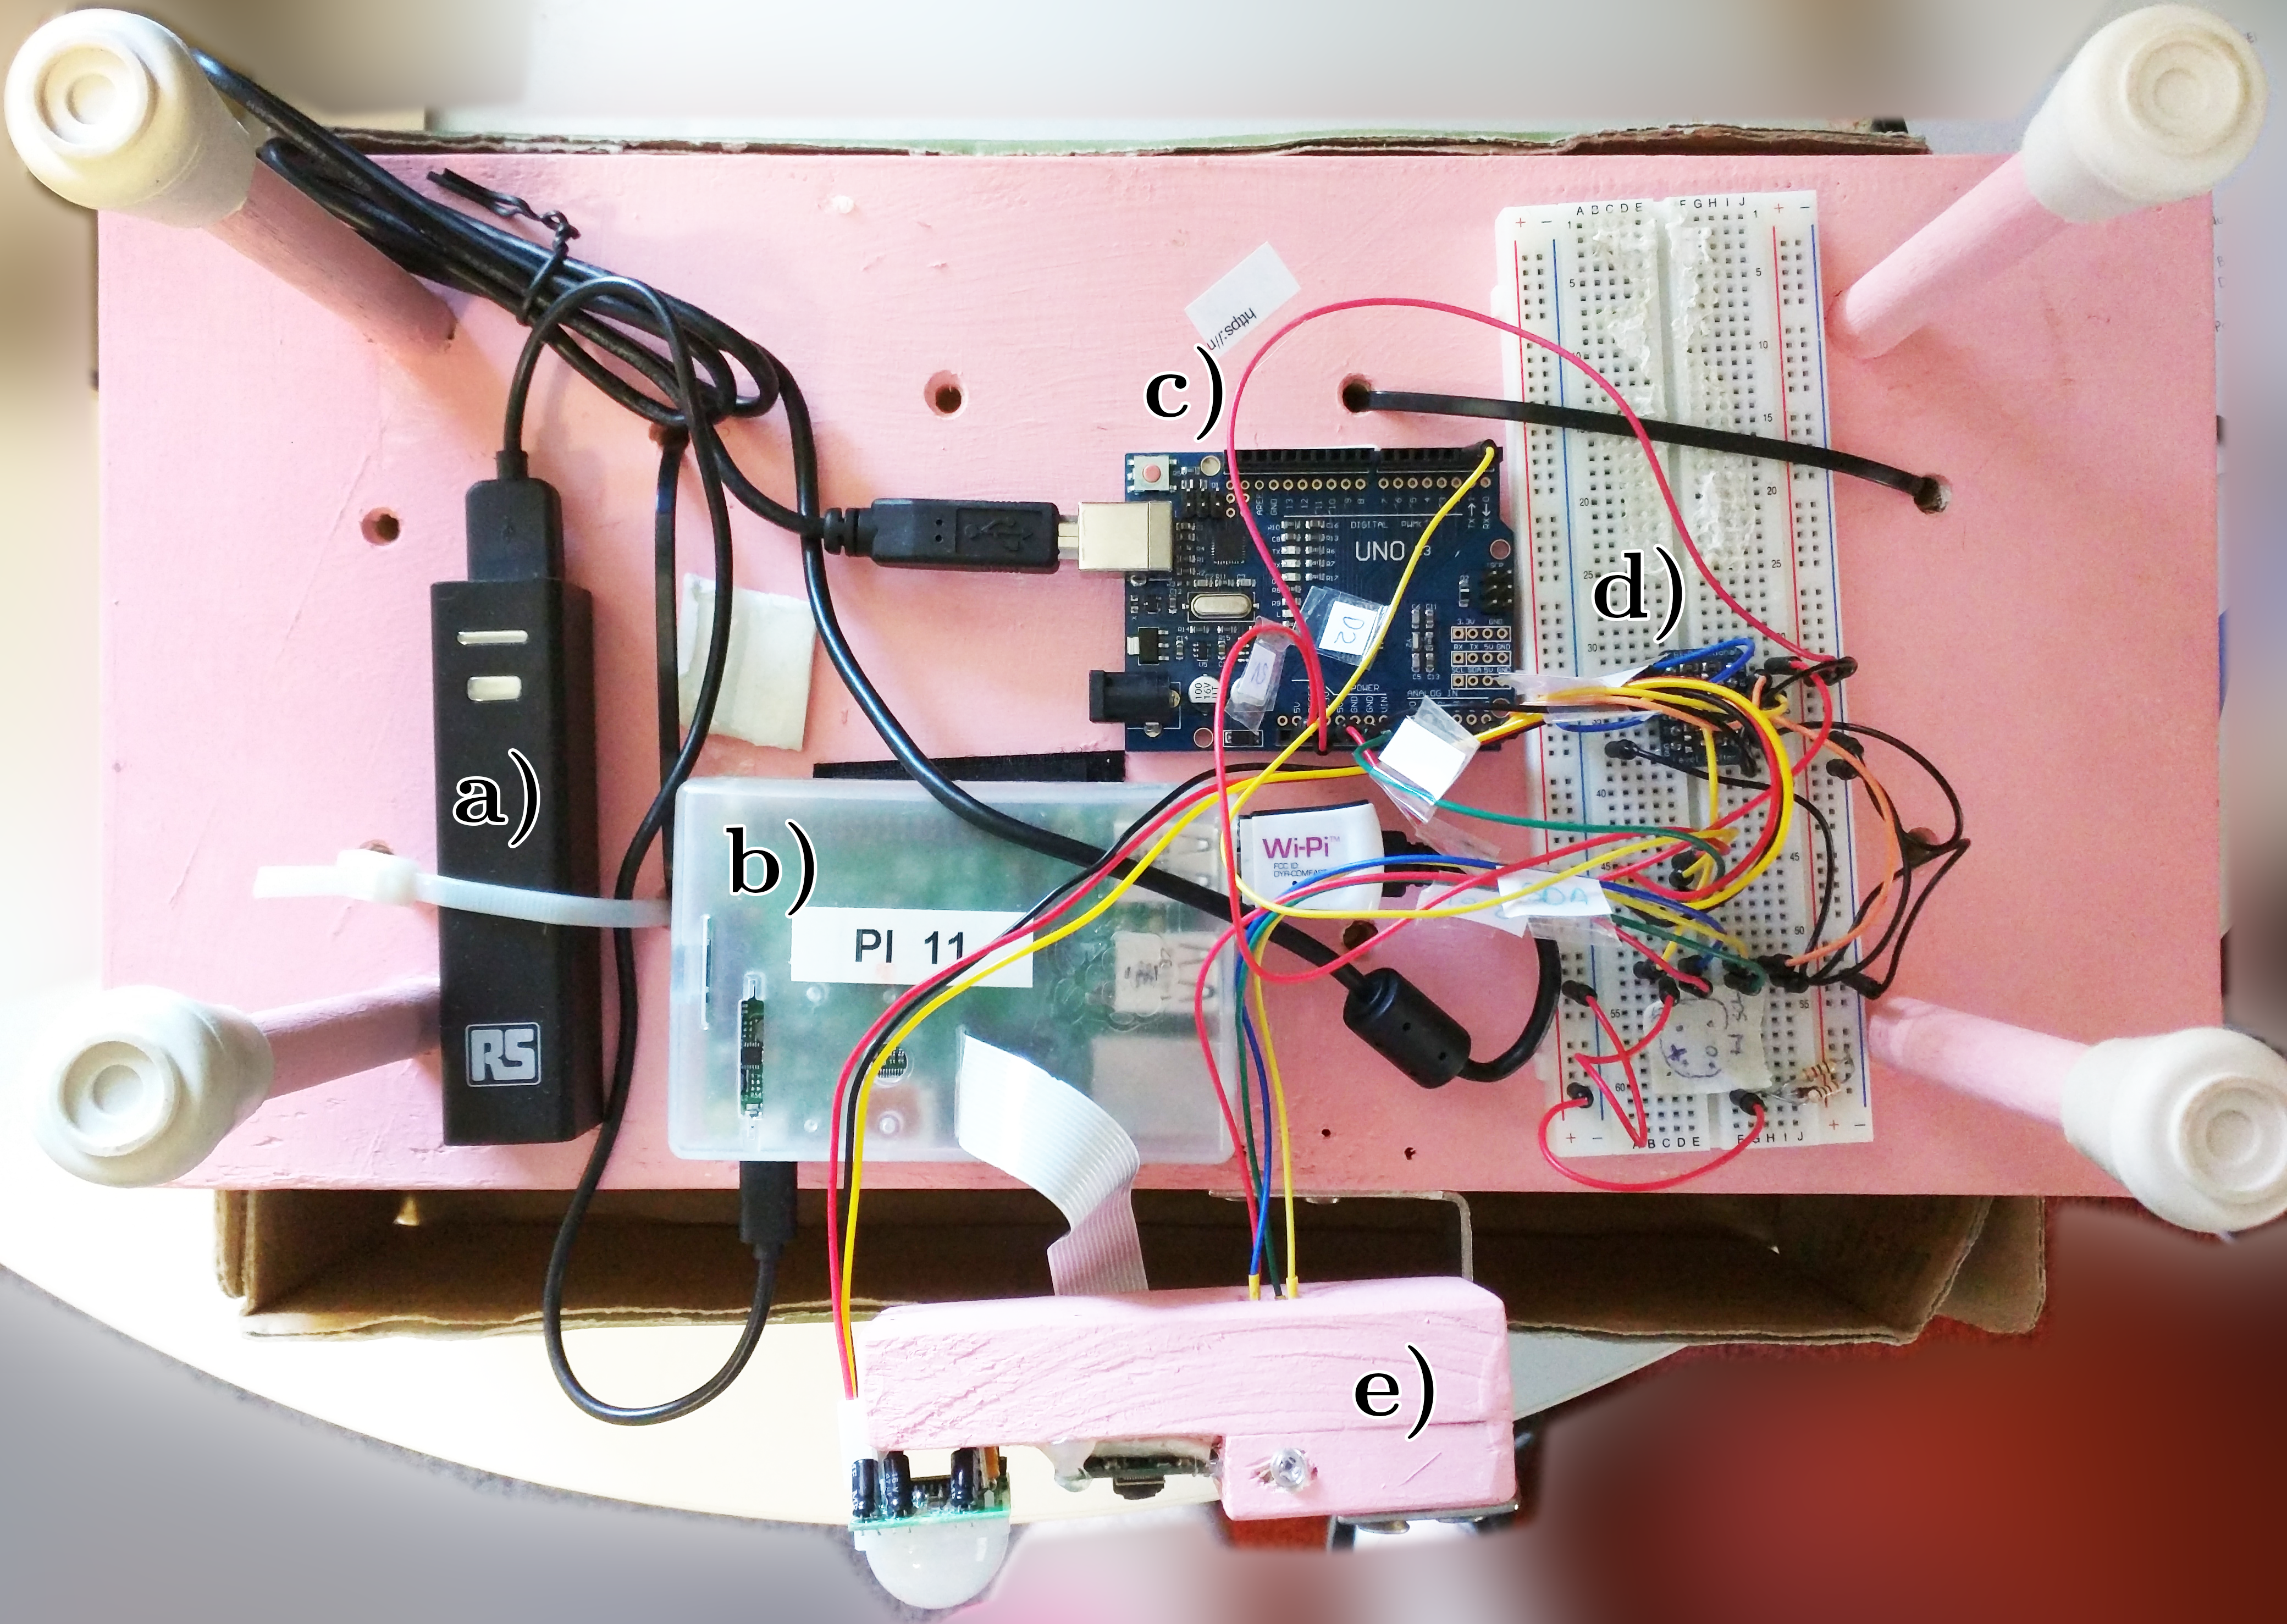
\includegraphics[width=\textwidth]{../diagrams/prototypeb-1.jpg}
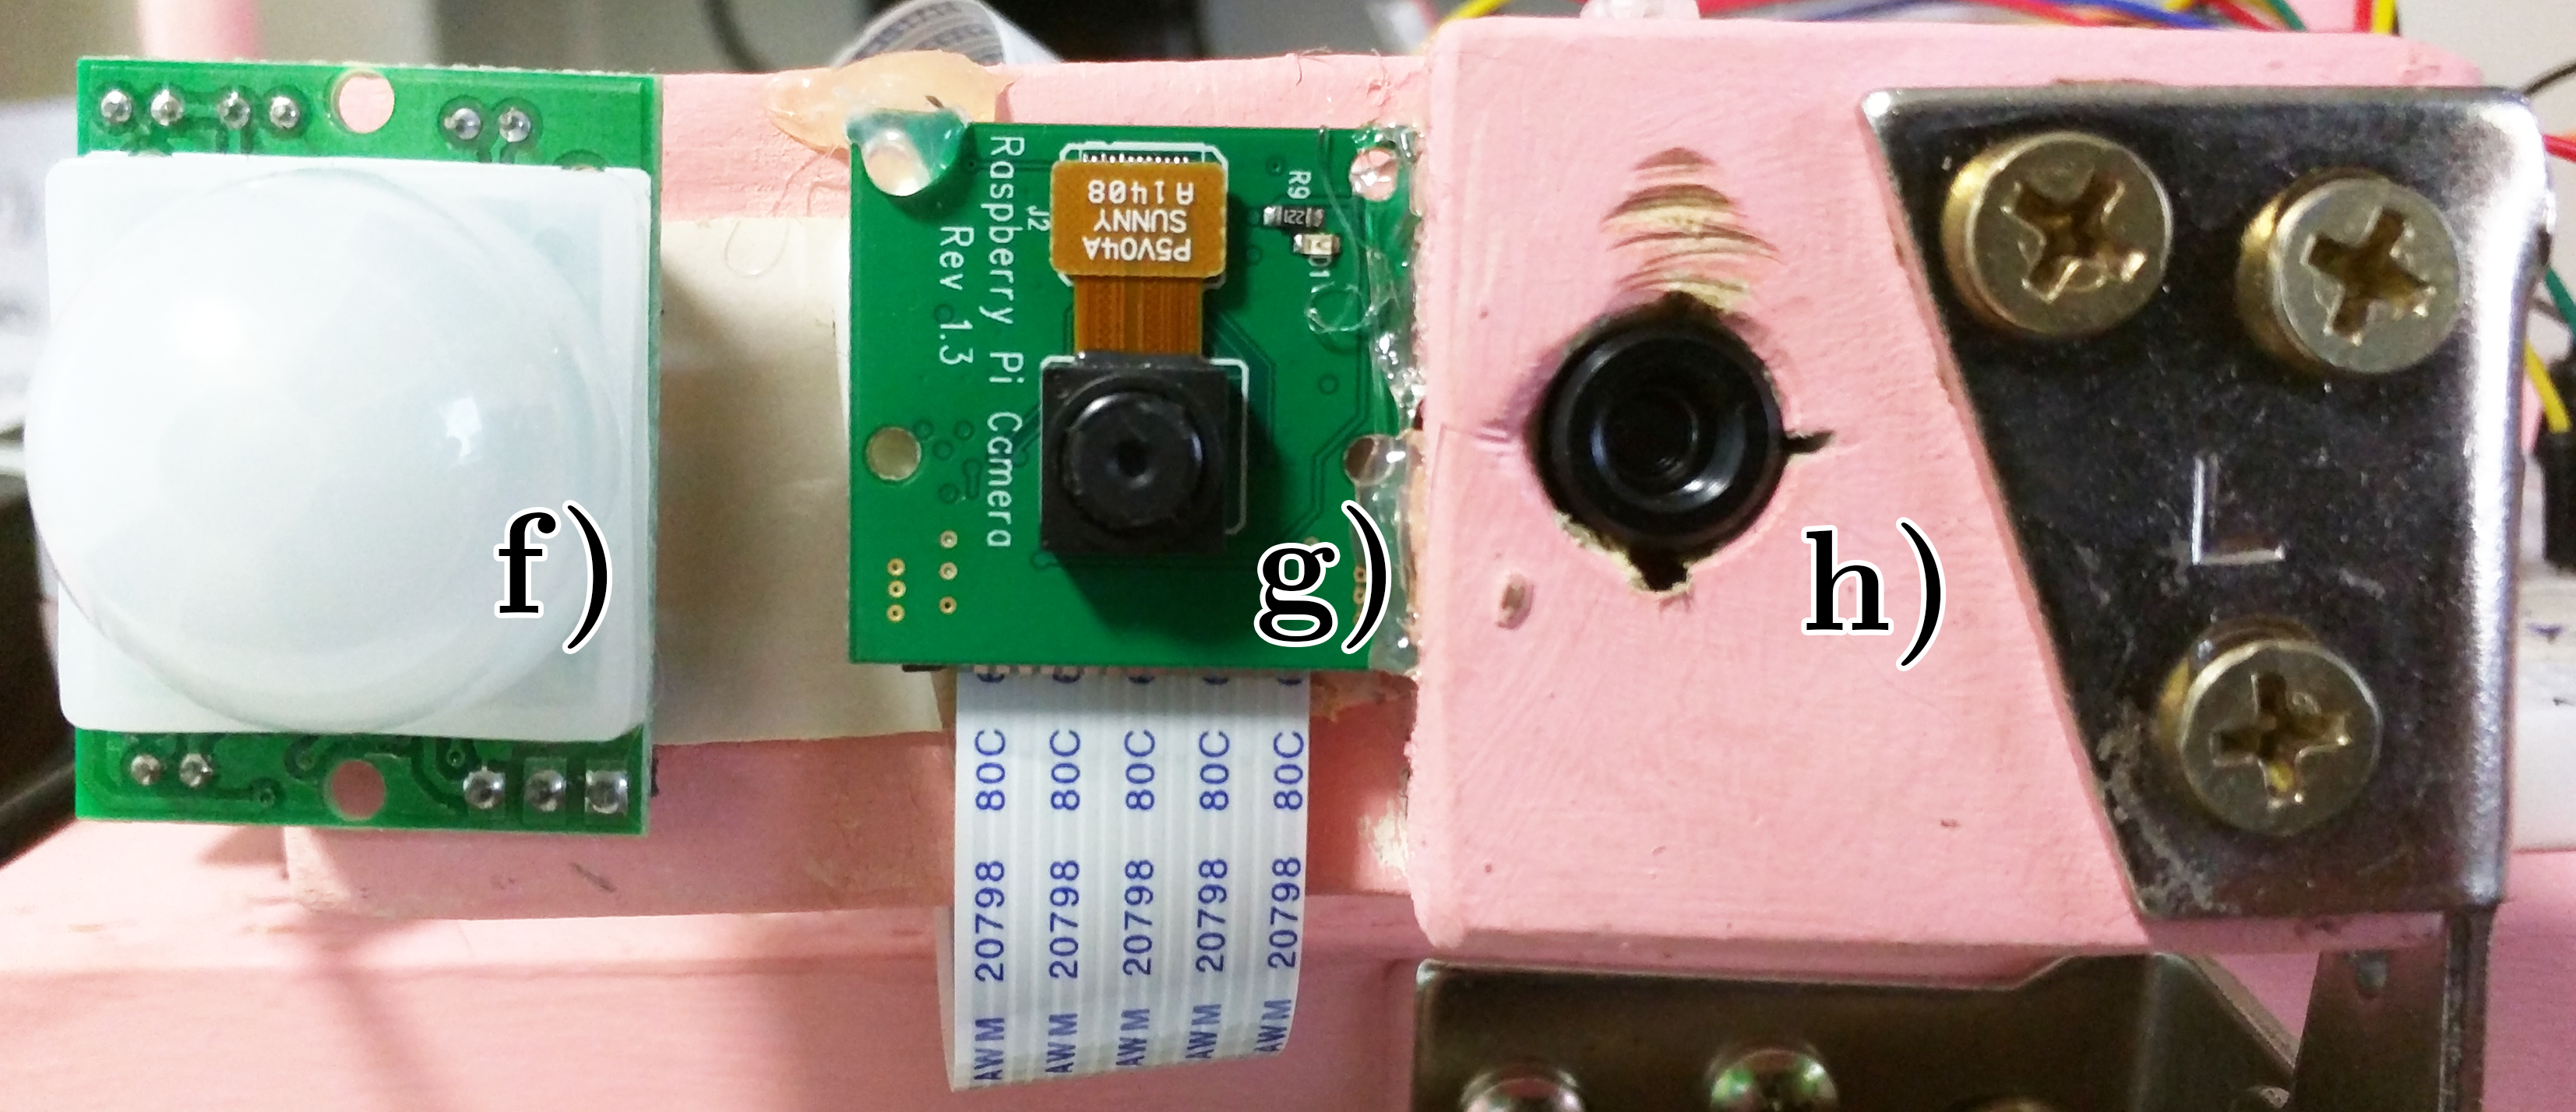
\includegraphics[width=\textwidth]{../diagrams/prototypeb-2.jpg}
{\small
\begin{multicols}{2}
\begin{enumerate}[a)]
 \item Battery pack
 \item Raspberry Pi
 \item Arduino
 \item Level-shifting circuitry
 \item Movable sensor mount
 \item PIR
 \item Camera
 \item \mlx
\end{enumerate}
\end{multicols}
}
\caption{Prototype Physical Form}
\label{fig:pictures:protob1}
\end{figure}

\chapter{Original Honours Proposal}
\subfile{../proposal/proposal}

%\clearpage



\end{document}


